\documentclass[12pt,a4paper]{standalone}
\usepackage[latin1]{inputenc}
\usepackage{amsmath}
\usepackage{amsfonts}
\usepackage{amssymb}
\usepackage{graphicx}
\usepackage{tikz}
\usetikzlibrary{decorations.markings}
\begin{document}
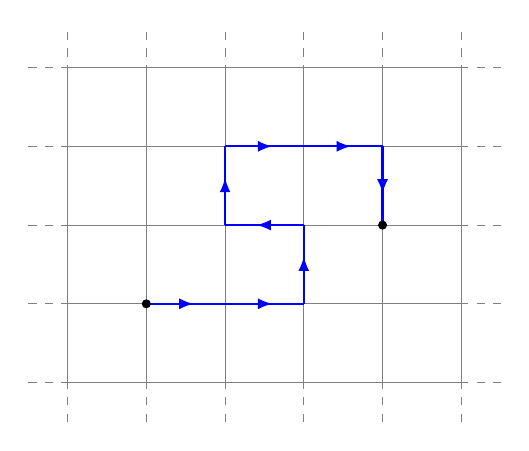
\begin{tikzpicture}
\tikzset{middlearrow/.style={decoration={markings,mark= at position 0.6 with {\arrow{#1}} ,},postaction={decorate}}};
\draw[step=1cm,color=gray,dashed] (-1.5,-1.5) grid (4.5,3.5);
    \draw[step=1cm,color=gray] (-1,-1) grid (4,3);
    \draw[middlearrow={latex},thick,blue] (0,0)--(1,0);
    \draw[middlearrow={latex},thick,blue] (1,0)--(2,0);
    \draw[middlearrow={latex},thick,blue] (2,0)--(2,1);
    \draw[middlearrow={latex},thick,blue] (2,1)--(1,1);
    \draw[middlearrow={latex},thick,blue] (1,1)--(1,2);
    \draw[middlearrow={latex},thick,blue] (1,2)--(2,2);
    \draw[middlearrow={latex},thick,blue] (2,2)--(3,2);
    \draw[middlearrow={latex},thick,blue] (3,2)--(3,1);
    \draw[fill] (0,0) circle (0.05);
    \draw[fill] (3,1) circle (0.05);
\end{tikzpicture}

\end{document}